% =============================================================================
% SECTION 5 -- FUNDAMENTALS: services, storage, and why text wins
% =============================================================================

\section{Fundamentals}
\subsection{Services}

% ---------------------------------------------------------------------------
% 5.1  how do you interact with computers?
% ---------------------------------------------------------------------------
\begin{frame}{How do you interact with computers?}{spoiler: services}
    \begin{center}
        \begin{tikzpicture}
            % you
            \node[circle,draw=neonyellow,very thick,minimum size=1.5cm,
                  text=neonyellow,font=\small\bfseries] (you) at (0,0) {You};
            % services
            \node[draw=accentcyan,rounded corners,fill=darkgray,align=center,
                  minimum width=2.7cm,minimum height=1.05cm] (g) at (3.7,2.25)
                  {
\includegraphics[height=0.45cm]{assets/img/google.png}\\[0.05em] {\tiny Google}};
            \node[draw=accentcyan,rounded corners,fill=darkgray,align=center,
                  minimum width=2.7cm,minimum height=1.05cm] (a) at (3.7,0)
                  {
\includegraphics[height=0.45cm]{assets/img/amazon.png}\\[0.05em] {\tiny Amazon}};
            \node[draw=accentcyan,rounded corners,fill=darkgray,align=center,
                  minimum width=2.7cm,minimum height=1.05cm] (b) at (3.7,-2.25)
                  {{\tiny bank} \\[-0.15em] {\tiny UPI $\cdot$ netbanking} \\[-0.15em] {\tiny services}};
            % retrieval hub
            \node[draw=neongreen,very thick,rounded corners,fill=darkgray,align=center,
                  text=neongreen,font=\small,minimum width=3.4cm,minimum height=1.5cm] (ir) at (7.8,0)
                  {Information\\[-0.1em] Retrieval\\[-0.1em]
                   {\tiny\color{softgray} retrieve $\cdot$ rank $\cdot$ present}};
            % outcome
            \node[draw=neonyellow,rounded corners,fill=darkgray,align=center,
                  text=neonyellow,font=\small,minimum width=2.7cm,minimum height=1.15cm] (out) at (11.4,0)
                  {Answers\\[-0.1em] {\tiny a better life}};
            % edges
            \draw[-{Stealth},thick,softgray] (you) -- node[above,font=\tiny]{query} (g);
            \draw[-{Stealth},thick,softgray] (you) -- node[above,font=\tiny]{query} (a);
            \draw[-{Stealth},thick,softgray] (you) -- node[above,font=\tiny]{query} (b);
            \draw[-{Stealth},thick,softgray] (g) -- (ir);
            \draw[-{Stealth},thick,softgray] (a) -- (ir);
            \draw[-{Stealth},thick,softgray] (b) -- (ir);
            \draw[-{Stealth},very thick,neongreen] (ir) -- (out);
        \end{tikzpicture}
    \end{center}
    \pause
    \begin{center}
        {\small Google, Amazon, even banks --- they are \glow{services}.\\
        What do services do? \glow{They retrieve information for you} --- and make your life better.}
    \end{center}
\end{frame}

% ---------------------------------------------------------------------------
% 5.2  side note: about me
% ---------------------------------------------------------------------------
\subsection{Side Note}

\begin{frame}{Side note: who's talking?}{about me}
    \begin{columns}
        \begin{column}{0.55\textwidth}
            \begin{tcolorbox}[darkstyle,title={\tiny Shuvam Banerji Seal}]
                {\small
                \textbf{BS--MS final-year student}, IISER Kolkata\\[0.1em]
                Chemistry major $\cdot$ Computer Science minor\\[0.2em]
                Research: \glow{Information Retrieval} --- RAG, BM25, TREC, ECIR'26\\[0.2em]
                Clubs: President, Slashdot $\cdot$ Office Bearer, Valence\\[0.2em]
                {\tiny\color{softgray} github.com/Shuvam-Banerji-Seal $\cdot$ shuvam-banerji-seal.github.io}
                }
            \end{tcolorbox}
        \end{column}
        \begin{column}{0.4\textwidth}
            \begin{itemize}[<+->]
                \item I study chemistry, I code for a living, I research \glow{retrieval}.
                \item I teach tools for fun --- like this talk.
                \item Everything I show you, I use daily.
            \end{itemize}
        \end{column}
    \end{columns}
\end{frame}

% ---------------------------------------------------------------------------
% 5.3  where does information live?
% ---------------------------------------------------------------------------
\subsection{Where Information Lives}

\begin{frame}{How is information stored in this digital era?}{you tell me}
    \begin{center}
        \glowtitle[neonyellow]{You tell me.}
    \end{center}
    \pause
    \begin{center}
        \begin{tikzpicture}
            \node[draw=softgray,rounded corners,fill=darkgray,align=center,
                  minimum width=3.6cm,minimum height=3.0cm] (v) at (0,0)
                  {
\includegraphics[height=0.9cm]{assets/img/youtube.png}\\[0.2em]
                   {\small Video}\\[0.1em] {\tiny\color{softgray} most of the bytes}};
            \node[draw=softgray,rounded corners,fill=darkgray,align=center,
                  minimum width=3.6cm,minimum height=3.0cm] (p) at (4.4,0)
                  {\resizebox{1.0cm}{!}{\begin{tikzpicture}
                       \draw[fgwhite,very thick] (0,0) rectangle (1.2,0.9);
                       \draw[fgwhite,very thick] (0.6,0.45) circle (0.22);
                       \draw[fgwhite,very thick] (0,0) -- (0.35,0.32) -- (0.6,0.15) -- (1.2,0.7);
                   \end{tikzpicture}}\\[0.2em]
                   {\small Photos}\\[0.1em] {\tiny\color{softgray} many bytes}};
            \node[draw=accentcyan,very thick,rounded corners,fill=darkgray,align=center,
                  minimum width=3.6cm,minimum height=3.0cm] (t) at (8.8,0)
                  {
\includegraphics[height=0.9cm]{assets/img/wikipedia.png}\\[0.2em]
                   {\small \textbf{Text}}\\[0.1em] {\tiny\color{neongreen} few bytes, most value}};
            % "?" above the audience answer
            \node[text=neonyellow,font=\large] at (4.4,2.2) {?};
        \end{tikzpicture}
    \end{center}
    \pause
    \begin{center}{\small out of the three --- \glow{text} is the one that constitutes all these services and softwares.}\end{center}
\end{frame}

% ---------------------------------------------------------------------------
% 5.4  it's all text
% ---------------------------------------------------------------------------
\subsection{It's All Text}

\begin{frame}{It's all text}{the universal interface}
    \begin{columns}
        \begin{column}{0.52\textwidth}
            \begin{itemize}[<+->]
                \item Out of \glow{video}, \glow{photos} and \glow{text} --- which one runs every service?
                \item \textbf{Text}. Text is the universal interface.
                \item Google? A text-index of the web. \quad Your bank? Text rows in a database.
                \item LLMs eat text. \glow[neongreen]{Agents act on text.}
            \end{itemize}
        \end{column}
        \begin{column}{0.44\textwidth}
            \begin{center}
                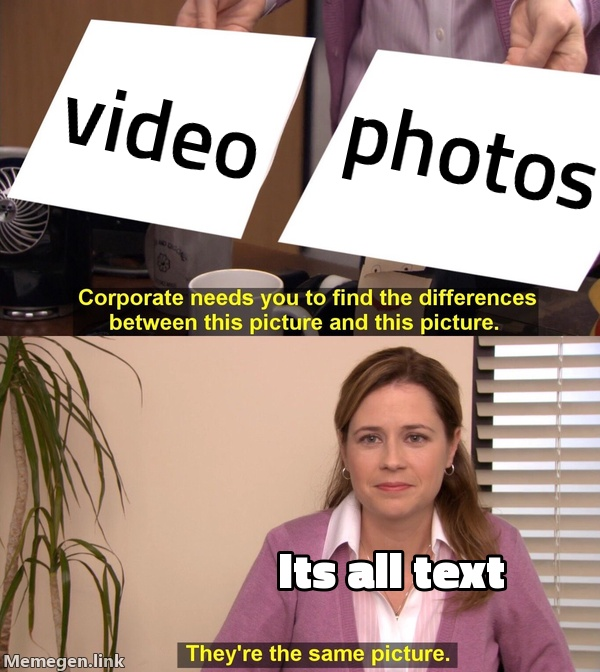
\includegraphics[height=3.0cm]{assets/img/meme_samepicture.jpg}\\[0.15em]
                \onslide<2->{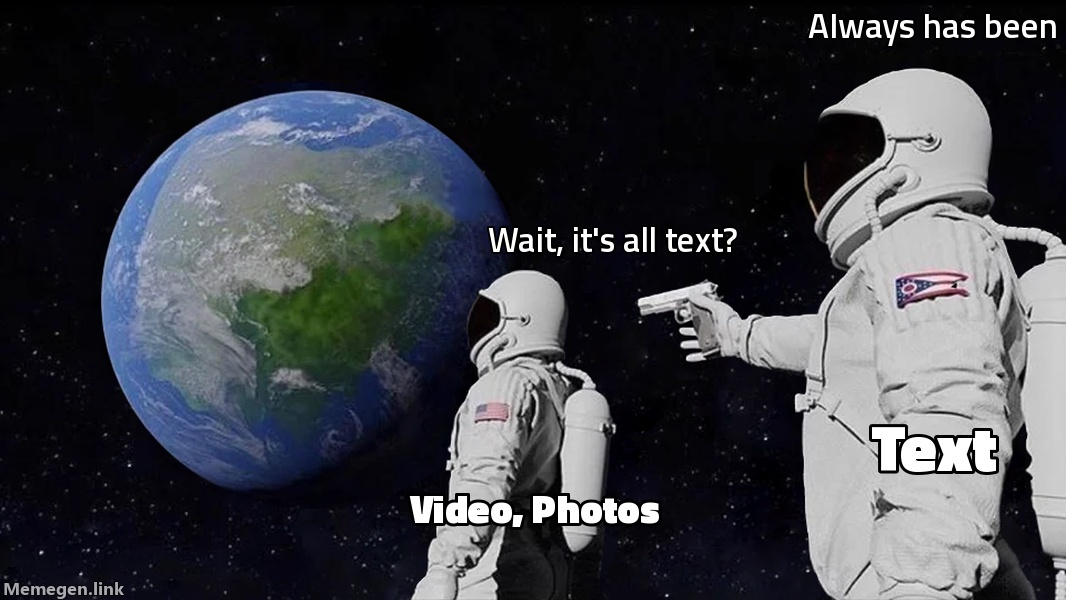
\includegraphics[height=2.7cm]{assets/img/meme_alwayshasbeen.jpg}}
            \end{center}
        \end{column}
    \end{columns}
\end{frame}
